\section{Planificació}
En aquesta secció es tractaran temes com la planificació temporal de les tasques, així com les desviacions sofertes al llarg del temps.
\subsection{Diagrama de Gantt}
Tot i la tipologia àgil de la planificació, s'ha intentat plasmar sobre un diagrama de Gantt les tasques descrites a la secció \ref{gestio:tasques}, i així representar el flux de treball que hauria de seguir el projecte durant el temps que aquest duri.\\
\newline Cada una de les caselles que es poden veure sobre el diagrama correspon a una de les tasques especificades a la secció \ref{gestio:tasques}.\\
\newline El diagrama en qüestió es pot trobar a la pàgina següent (Figura \ref{fig:Gantt}).\\
\subsubsection{Consideracions}
Per a interpretar correctament el diagrama,  cal tenir en compte que mostra dos planificacions d'un mateix projecte, ``Planificació incicial'' i ``Planificació real''.\\
L'objectiu de representar-les de forma conjunta és permetre una comprensió global de l'avanç real del projecte en el temps, tenint en compte les desviacions sofertes durant el desenvolupament.\\
\newline En el Gantt inferior, corresponent al cas real, es poden apreciar tres colors.\\
El primer, blau, igual que la planificació superior, correspon a aquelles tasques que no s'han vist afectades per les desviacions.\\
Seguidament, en groc es representa un període, fruit de problemes sorgits en el desenvolupament (es donaran més detalls en capítols posteriors), i que obliguen a prendre aquest temps per investigar i replantejar el rumb a seguir.\\
Finalment, en verd es mostren les tasques sorgides de la revisió i re-planificació del projecte.\\
\newline S'ha inclòs una tasca referent a la redacció d'aquesta memòria, ja que es considera que forma part del projecte. En el cas del segon Gantt, la memòria s'ha vist finalitzada fora del plaç establert.

%\newline Addicionalment, s'ha afegit una tasca (també especificada a la secció \ref{gestio:tasques}) corresponent a la redacció d'aquesta memòria.
%Tot i l'ús \textit{kanban} com a metodologia de planificació del projecte, s'ha intentat estimar les tasques en funció de la seva complexitat aproximada, per intentar predir l'evolució del projecte.\\
%\newline El diagrama de Gantt que es mostra a continuació s'ha d'interpretar com si de dos diagrames de Gantt diferents
\begin{landscape}
\begin{figure}[ht]
\begin{center}
\vspace{2cm}
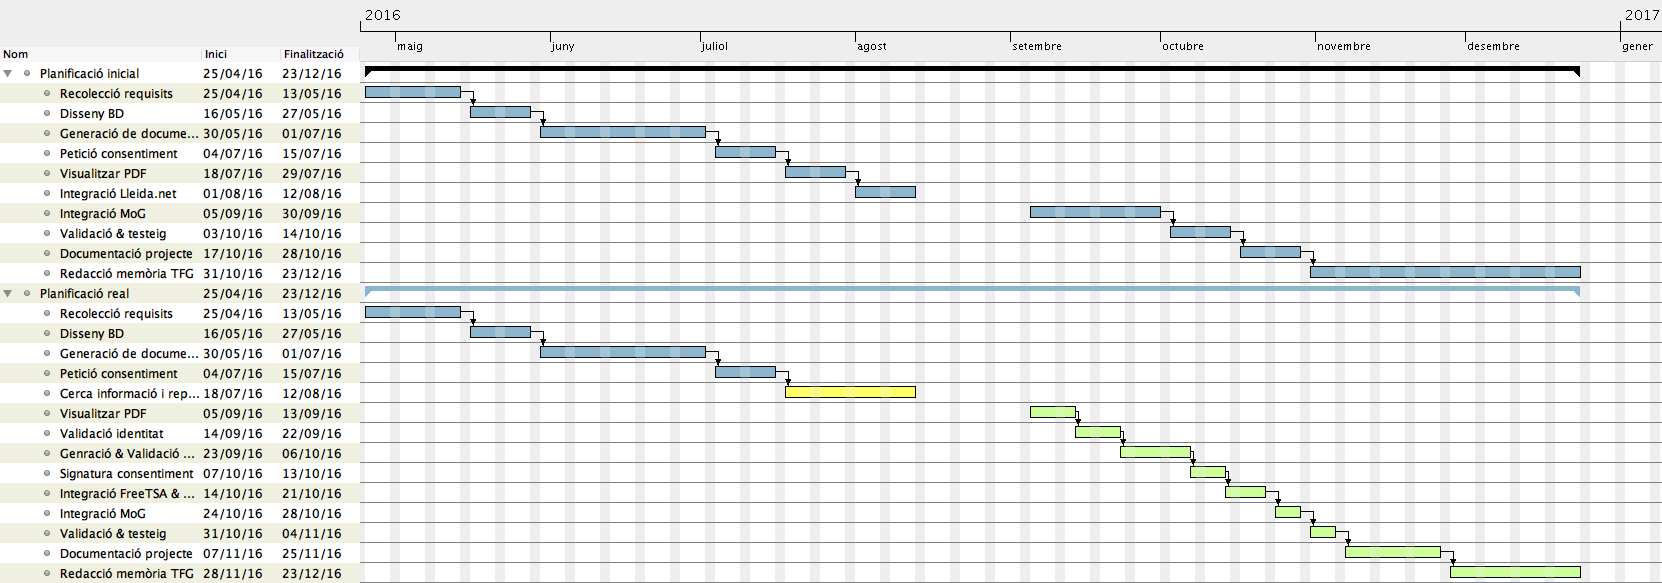
\includegraphics[scale=0.4]{sections/gestio/tfg-gantt.png}
\end{center}
\caption{Diagrama de Gantt}
\label{fig:Gantt}
\end{figure}
\end{landscape}
%\includegraphics[scale=0.5]{sections/gestio/GanttHPart1.png}	
%\includegraphics[scale=0.5]{sections/gestio/GanttHPart2.png}	

%\subsection{Interpretació}
%Com es pot apreciar al diagrama anterior, la planificació està prevista per a que el projecte, començant juntament amb el conveni el 25 d'abril d'aquest mateix any, finalitzi en acabar l'any.\\
%\newline Dins del projecte, tal i com es pot haver apreciat durant l'explicació de les tasques, podem trobar tres fases clarament diferenciades.
%\renewcommand{\labelenumi}{\roman{enumi}}
%\begin{enumerate}
%	\item En aquesta primera part, marcada en el diagrama de Gantt anterior amb color blau, es pretén assentar les bases per al posterior desenvolupament, adquirir tots, o si més no gran part,  els coneixements necessaris per a dur a bon port el futur desenvolupament.\\
%		\newline En aquesta primera fase s'inclou, la lectura i anàlisi de les diferents lleis sobre signatura, investigació sobre possibles tecnologies i camins a seguir, així com agafar una mica de rodatge amb les tecnologies emprades dins de la pròpia empresa.
%	\item Seguidament, marcada a la figura anterior de color vermell, el gruix del projecte. Tot el desenvolupament on s'han d'aplicar tots els coneixements adquirits durant el transcurs de la fase anterior.\\
%		\newline Aquesta fase inclou tot el procés de desenvolupament i testeig del mòdul, així com la seva posterior integració a la plataforma i el seu corresponent testeig.
%	\item Finalment, es pot apreciar de color verd, a la figura anterior, una fase que comença a mitjans de la fase de cerca: el procés de documentació.\\
%		\newline És important que es documenti a mesura que es desenvolupa per tal del mantenir la informació al dia, i que en un futur, la informació emmagatzemada dins d'aquesta documentació no sigui fruit del record del moment sobre una decisió concreta.
%\end{enumerate}

\subsection{Desviacions}
%Com en tot projecte, existeix la possibilitat de que sorgeixin desviacions que fan que els temps pensats inicialment no es compleixin.\\
%Per pal·liar aquestes possibles desviacions, es contemplen tres possibles accions inicials:
%\begin{itemize}
%	\item \textbf{Ampliació de l'equip de desenvolupament}\\
%Aquesta opció, tal i com indica el seu nom, consisteix en la contractació de nous desenvolupadors, ja sigui amb un caràcter definitiu o temporal, per tal de reforçar l'equip i permetre assolir les diferents tasques que formen el projecte més ràpidament i amb una major solvència.\\
%	\item \textbf{Aplaçar la data final de lliurament}\\
%Al tractar-se d'un Treball de Final de Grau, la data d'entrega queda estipulada des d'un primer moment amb la intenció de fitar el projecte dins del quadrimestre corresponent; per altra banda, la finalització del conveni amb l'empresa també dictamina una data límit.\\
%	\item \textbf{Reformular els requisits del projecte}\\
%Finalment, la última opció que es planteja consisteix en reformular el plantejament inicial del que hauria de ser el projecte acabat, amb la idea d'eliminar aquelles \textit{features} que no siguin estrictament necessàries i vitals per al bon funcionament d'aquest i que no siguin claus per a la seva posterior integració amb la plataforma.\\
%\end{itemize}
%De totes les opcions presentades, la que sembla que més viabilitat té dins dels plantejament que es dóna al projecte és la tecera, que planteja un reformulació del projecte, tenint sempre com a objectiu, obtenir un mínim producte viable que compleixi amb els requeriments i necessitats bàsiques de la plataforma.
Al llarg del projete han sorgit imprevistos, que n'han endarrerit el desenvolupament, però que per sort no han evitat que es desenvolupés dins del temps estipulat en un primer moment.\\
\newline Els imprevistos en qüestió, sobre els quals es donen detalls en capítols posteriors, tenen a veure amb el procés d'integració d'aquest projecte de final de grau amb els serveis oferts per un tercer de confiança.\\
\newline Aquest imprevist, de caràcter aparentment lleu, ha resultat en un replantejament global del funcionament i de les mecàniques del projecte.\\
\newlien Un cop resolta la incidència i replantejat el projecte, la planificació s'ha complert sense més incidents.
